For example, the $n = 10$ Fig. \ref{210f}, the formula as follows:

\begin{figure}[h]
\centering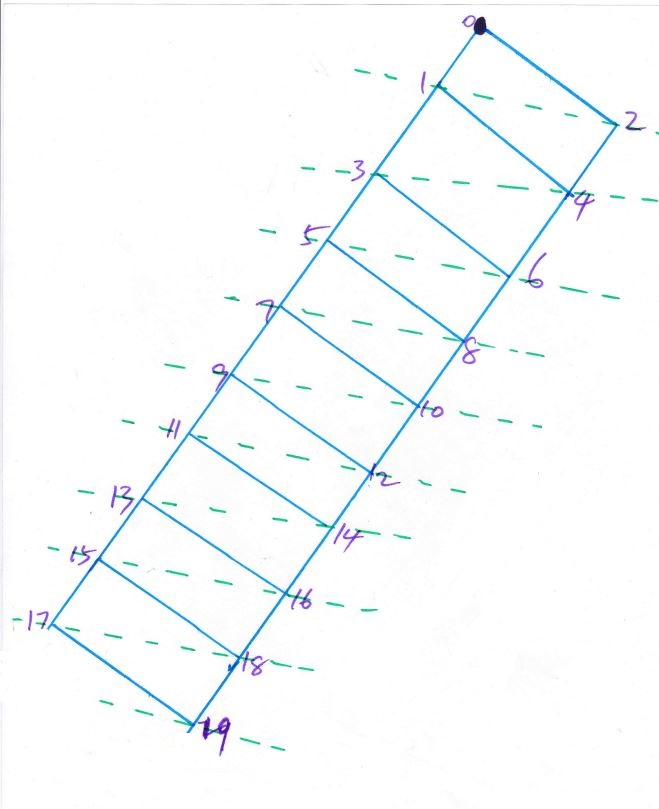
\includegraphics[width=0.7\linewidth]{figure/c210_f}
\caption{2*n $(n = 10)$ regular mesh}
\label{210f}
\end{figure}


\begin{equation}
{
\left[ \begin{array}{ccccccc}
1 & 2 & 2 & \cdots & 2 & 2 & 1\\
1 & -1 & 0 & \cdots& 0 & 0 & 0\\
0 & \sigma-1 & 1 & \cdots & 0 & 0 & 0 \\
0 & \sigma-1 & \sigma & 1 & 0 & \cdots & 0 \\
0 & \sigma-1 & \sigma & \sigma & 1 & 0 & 0 \\
\vdots & \vdots & \vdots  &   \vdots & \ddots & \ddots\\
0 & \sigma-1 & \sigma & \cdots & \sigma & \sigma & 1
\end{array} 
\right ]} \times \left[ \begin{array}{c}
\alpha_{0} \\
\alpha_{1} \\
\alpha_{3} \\
\alpha_{5} \\
\vdots \\
\alpha_{2 \times n - 1}\\
\alpha_{2 \times n + 1}
\end{array} 
\right ] = \left[ \begin{array}{c}
1 \\
0 \\
0 \\
0 \\
\vdots \\
0
\end{array} 
\right ]
\end{equation}

So the Speedup is $$\frac{1}{\alpha_{0}}$$.
\vspace*{50pt}
